\documentclass{standalone}

\usepackage{tikz}
\usetikzlibrary{chains,fit,shapes}

\begin{document}

\begin{tikzpicture}
\tikzstyle{every path}=[very thick]

\tikzstyle{tmtape}=[draw]

%% Draw TM tape
\begin{scope}[start chain=1 going right,node distance=5mm,every join/.style={-latex, very thick}]
    \node [on chain=1,tmtape,circle] {$\varepsilon_0$};
    \node [on chain=1,tmtape,draw=none,join] {$\ldots$};
    \node [on chain=1,tmtape,join] {
      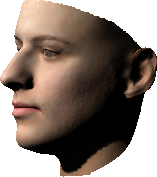
\includegraphics[height=2cm]{../images/trees/profile}
    };
    \node [on chain=1,tmtape,join] {
      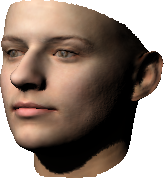
\includegraphics[height=2cm]{../images/trees/3-4}
    };
    \node [on chain=1,tmtape,join] {
      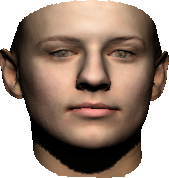
\includegraphics[height=2cm]{../images/trees/frontal}
    };
    \node [on chain=1,tmtape,join] {
      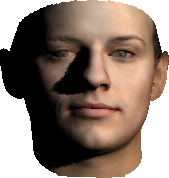
\includegraphics[height=2cm]{../images/trees/frontal-shaded}
    };
    \node [on chain=1,tmtape,draw=none,join] {$\ldots$};
\end{scope}

\end{tikzpicture}

\end{document}
